\documentclass[12pt, letterpaper]{article}
\usepackage[utf8]{inputenc}
\usepackage{cite}
\usepackage{float}
\usepackage{tikz}
\usepackage{hyperref}
\usepackage[newfloat]{minted}
\usepackage{caption}
\usepackage{dirtree}
\tolerance=1
\emergencystretch=\maxdimen
\hyphenpenalty=10000
\hbadness=10000

\newenvironment{code}{\captionsetup{type=listing}}{}
\SetupFloatingEnvironment{listing}{name=Source Code}

\graphicspath{{img/}}

\title{Simulation of TLS (42)}
\author{Leskovar Lukas Andreios (KatNr), 5BHIF}
\date{March 2022}

\begin{document}

\begin{titlepage}
\maketitle
\end{titlepage}

\tableofcontents
\newpage

\section{Introduction}
The goal of this project was to simulate communication over Transport Layer Security (TLS) by implementing the Diffie-Hellman Internet Key Exchange (IKE). Any further communication was to be encrypted by a symmetric encryption algorithm.

\section{Transport Layer Security}
The nowadays de-facto standard for communicating over the internet is Transport Layer Security. Its predecessor SSL was replaced by TLS 1.0 in 1999. In 2018 the newest version 1.3 was implemented which drastically reduced the overhead during handshakes.

\subsubsection{Key Generation}


\subsubsection{Handshake}


\section{Software Architecture}

\subsection{Technologies}

\begin{table}[h]
	\centering
	\begin{tabular}{l|l}
		Purpose                       & Technology \\ \hline
		Build Tool				 	  & Meson	   \\
		Command line interface	      & CLI11      \\
		Configuration files           & json       \\
		Data serialization            & Protobuf   \\
		Logging                       & spdlog     \\
		Network Communication         & asio       \\
		Programming Languages		  & C++ 17 \\
		Encryption 					& plusaes \\
		Hashing 					& PicoSHA2 \\
		Large Integer Values & BigInt \\
	\end{tabular}
	\caption{This table lists all the technologies used in this project.}
\end{table}

\subsection{Classes}

\subsubsection{Communication}
The following classes are utilized by any other part of the application trying to send or receive messages over TCP.

\begin{figure}[H]
	\centering
	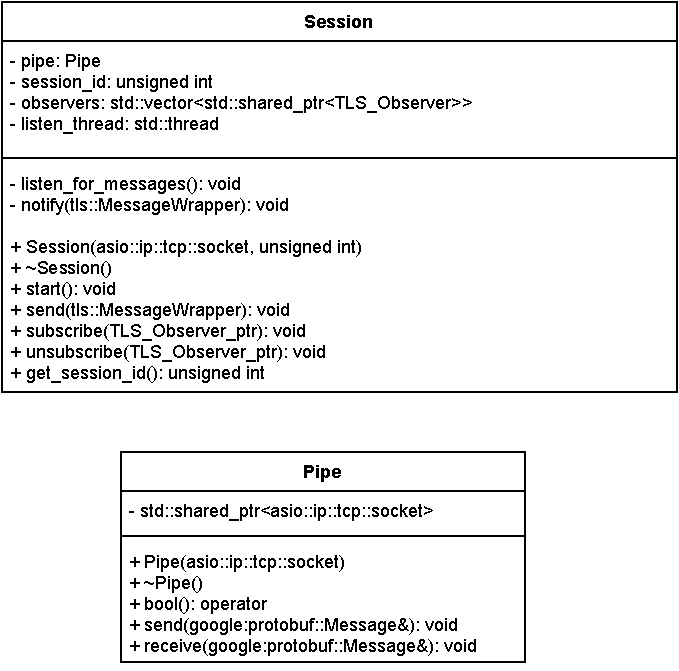
\includegraphics[width=.6\textwidth]{UML/CommunicationClasses}
	\caption{UML Diagram on the Session and Pipe classes used for communication.}
	\label{fig:CommunicationClasses}
\end{figure}

\begin{figure}[H]
	\centering
	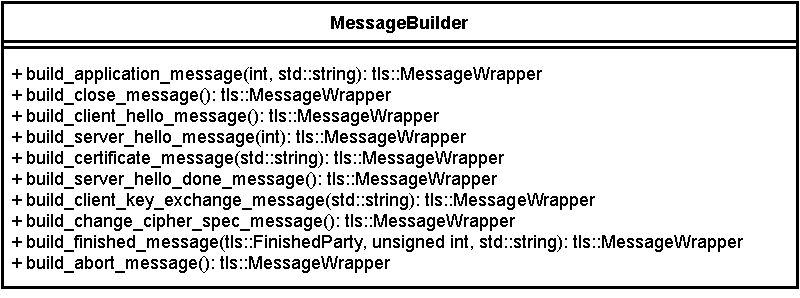
\includegraphics[width=.7\textwidth]{UML/Messagebuilder}
	\caption{The MessageBuilder is a utility class consisting of multiple static methods building Protobuf Messages.}
	\label{fig:Messagebuilder}
\end{figure}

\subsubsection{Main Logic}
To notify any main classes of new messages the observer pattern is implemented. The following classes each implement the TLS\_Observer and get notified by their respective session object once any messages are receives.

\begin{figure}[H]
	\centering
	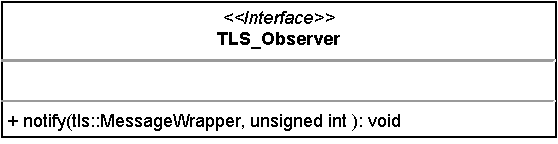
\includegraphics[width=.7\textwidth]{UML/Observer}
	\caption{The TLS\_Observer class implemented by any receiving class.}
	\label{fig:Observer}
\end{figure}

\begin{figure}[H]
	\centering
	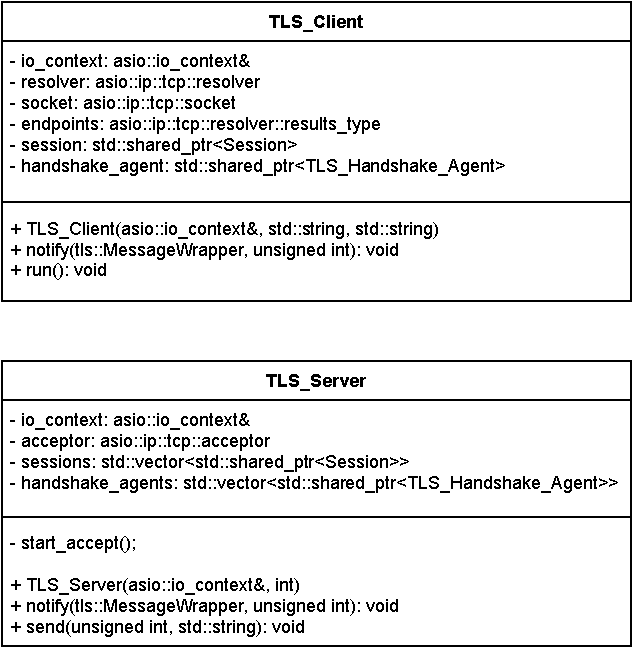
\includegraphics[width=.7\textwidth]{UML/ClientServer}
	\caption{The TLS\_Client and TLS\_Server classes containing main logic for the application.}
	\label{fig:ClientServer}
\end{figure}

\begin{figure}[H]
	\centering
	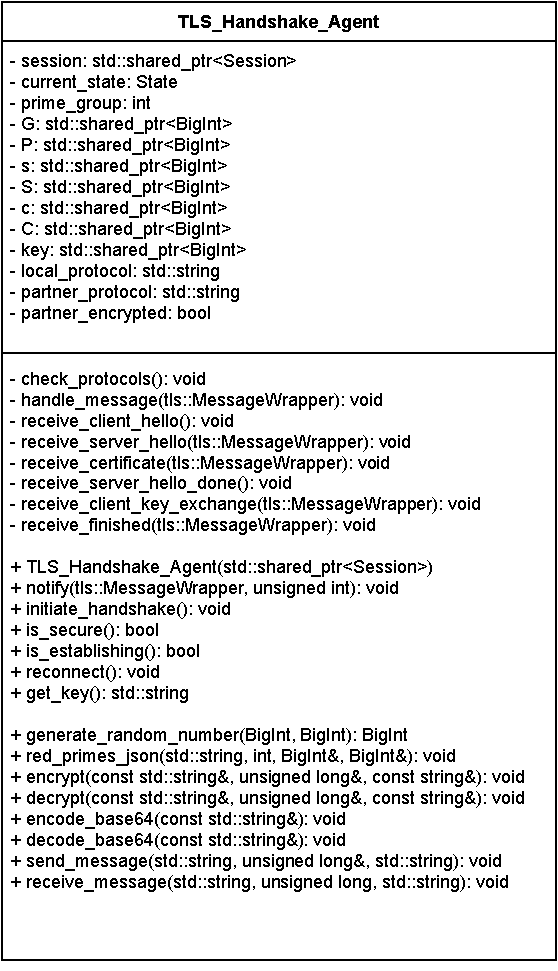
\includegraphics[width=.7\textwidth]{UML/HandshakeAgent}
	\caption{The TLS\_Handshake\_Agent handles any key exchange messages. It also contains  utility methods for encrypting/decrypting messages.}
	\label{fig:HandshakeAgent}
\end{figure}

\subsection{Class Association}

\begin{figure}[H]
	\centering
	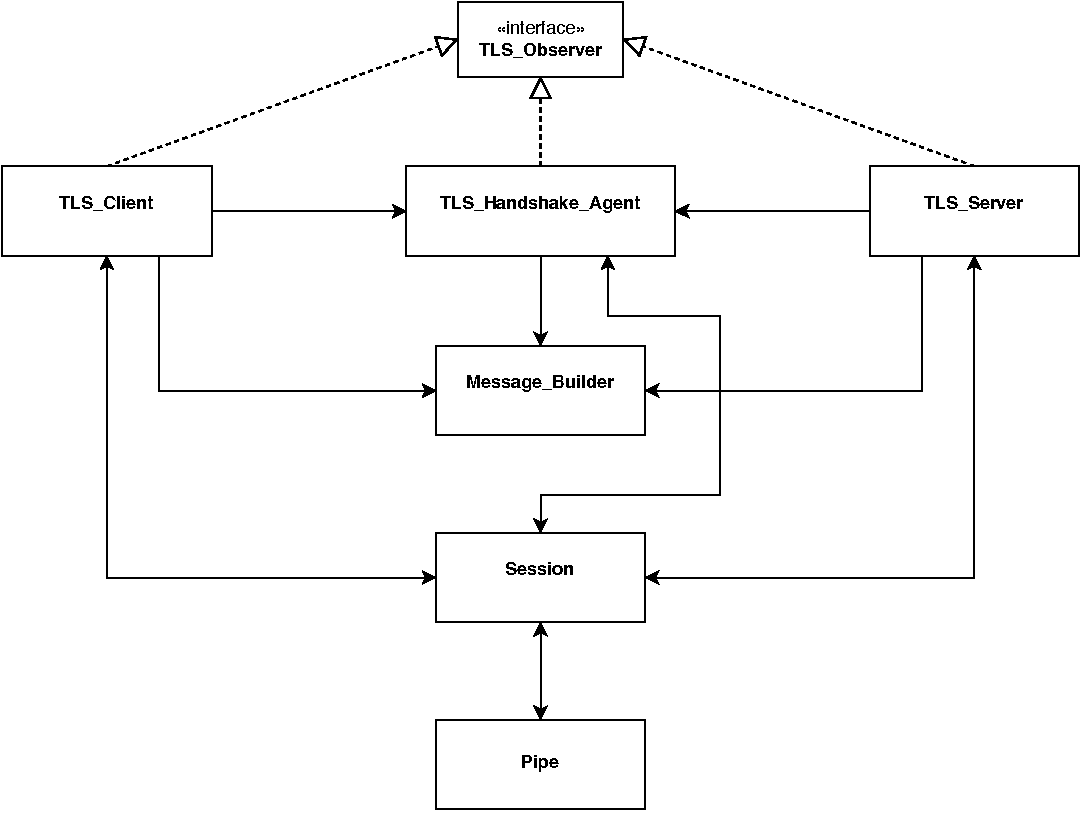
\includegraphics[width=.7\textwidth]{UML/ClassInteraction}
	\caption{This UML diagram shows how the different classes of the application are associated to each other.}
	\label{fig:ClassInteraction}
\end{figure}


\section{Description of code-blocks}


\subsection{Asio}
Network communication between client and server is established by utilizing asio.

\subsubsection{Client Connection}

\begin{code}
	\begin{minted}{cpp}
asio::io_context io_context;
asio::ip::tcp::resolver resolver(io_context);
asio::ip::tcp::socket socket(io_context);
asio::ip::tcp::resolver::results_type endpoints = 
  resolver.resolve(host, port);

asio::connect(socket, endpoints);

	\end{minted}
	\caption{Creation of socket connection on client side.}
	\label{clientConnection}
\end{code}

\pagebreak

\subsubsection{Server Connection}

\begin{code}
	\begin{minted}{cpp}
asio::io_context io_context{1};
asio::ip::tcp::acceptor acceptor{
  io_context, asio::ip::tcp::endpoint(asio::ip::tcp::v4(), port)
};
acceptor.async_accept(
[this](const std::error_code& ec, asio::ip::tcp::socket socket) {
  if (!ec) {
    // handle socket
  } else {
    // throw error
  }
});
	\end{minted}
	\caption{Server asynchronously waiting for client connections.}
	\label{serverConnection}
\end{code}

\subsection{Protobuf}
Any data to be sent over TCP is serialized using Google Protobuf \cite{protobuf}.

\subsubsection{Message Serialization}
\begin{code}
	\begin{minted}{cpp}
void Pipe::send(google::protobuf::Message& message) {
  u_int64_t message_size{message.ByteSizeLong()};
  asio::write(*socket, asio::buffer(&message_size, sizeof(message_size)));
	
  asio::streambuf buffer;
  std::ostream os(&buffer);
  message.SerializeToOstream(&os);
  asio::write(*socket, buffer);
}
	\end{minted}
	\caption{Serialization of protobuf messages.}
	\label{pipeSend}
\end{code}

\subsubsection{Message De-serialization}
\begin{code}
	\begin{minted}{cpp}
void Pipe::receive(google::protobuf::Message& message) {
  u_int64_t message_size;
  asio::read(*socket, asio::buffer(&message_size, sizeof(message_size)));
	
  asio::streambuf buffer;
  asio::streambuf::mutable_buffers_type bufs = buffer.prepare(message_size);
  buffer.commit(asio::read(*socket, bufs));
	
  std::istream is(&buffer);
  message.ParseFromIstream(&is);
}
	\end{minted}
	\caption{De-serialization of protobuf messages.}
	\label{pipeReceive}
\end{code}


%Pipe Klasse 

\subsection{TLS Handshake}
Whenever a new message is received the TLS\_Handshake\_Agent class is responsible for handling and responding to any handshake related message.

\subsection{Message Handling}

\begin{code}
	\begin{minted}{cpp}
void TLS_Handshake_Agent::handle_message(tls::MessageWrapper message) {    
  tls::MessageType messageType = message.type();
	
  if (messageType == tls::MessageType::CLIENT_HELLO) {
    receive_client_hello();
    
  } else if (messageType == tls::MessageType::SERVER_HELLO) {
    receive_server_hello(message);
		
  } else if (messageType == tls::MessageType::CERTIFICATE) {
    receive_certificate(message);
		
  } else if (messageType == tls::MessageType::SERVER_HELLO_DONE) {
    receive_server_hello_done();
		
  } else if (messageType == tls::MessageType::CLIENT_KEY_EXCHANGE) {
    receive_client_key_exchange(message);
	
  } else if (messageType == tls::MessageType::CHANGE_CIPHER_SPEC) {
    partnerEncrypted = true;
		
  } else if (messageType == tls::MessageType::FINISHED) {
    if (!partnerEncrypted) {
      session->send(Messagebuilder::build_abort_message());
      throw std::runtime_error("Partner did not send ChangeCipherSpec");
    }
    receive_finished(message);
		
  } else if (messageType == tls::MessageType::ABORT) {
    currentState = State::UNSECURED;
    throw new std::runtime_error("TLS connection aborted");
  } else {
    spdlog::error("Unknown message type: {}", messageType);
  }
}
	\end{minted}
	\caption{TLS Handshake Agent handling a message.}
	\label{messageHandling}
\end{code}


\subsection{External Libraries}
\label{extBib}

\subsubsection{CLI11}
CLI11 \cite{cli11_ref} implements a basic Command Line Interface (CLI) where users are able to specify parameters relevant for the program. 


\subsubsection{spdlog}
To log important information the logging library spdlog \cite{spdlog_ref} is employed.

\begin{code}
	\begin{minted}{cpp}
spdlog::trace("Trace bugs during development");
spdlog::debug("Debug messages");
spdlog::info("User-facing messages");
spdlog::warn("Potential errors");
spdlog::error("Errors");
spdlog::critical("Critical errors");
	\end{minted}
	\caption{Usage of different log types.}
	\label{spdlog}
\end{code}



\subsubsection{JSON}
Any further information, e.g. prime number for Diffie-Hellman IKE, is stored in a .json file which is read as follows. This is done using nlohman/json \cite{json_ref}.

\begin{code}
	\begin{minted}{cpp}
void TLS_Handshake_Agent::read_primes_json(
  std::string filename, 
  int id, 
  BigInt& g, 
  BigInt& p
) {
  std::ifstream file(filename);
  if (!file.is_open()) {
    throw new std::runtime_error("Error opening file");
  }
  nlohmann::json primes;
  file >> primes;
  file.close();
  g = int(primes["groups"][id]["g"]); 
  p = std::string(primes["groups"][id]["p_dec"]);
}
	\end{minted}
	\caption{nlohman reading the generator $g$ and prime number $p$.}
	\label{json}
\end{code}


\subsubsection{plusaes}
The header-only library plusaes \cite{plusaes} is used to symmetrically encrypt/decrypt messages.

\begin{code}
	\begin{minted}{cpp}
std::vector<unsigned char> key(32);
	
size = plusaes::get_padded_encrypted_size(message.size());
std::vector<unsigned char> encrypted(size);
	
plusaes::encrypt_cbc(
  (unsigned char*)message.data(), message.size(), 
  &key[0], key.size(), 
  &iv, 
  &encrypted[0], encrypted.size(), 
  true
);

	\end{minted}
	\caption{Plusaes encrypting a message}
	\label{plusaes}
\end{code}

\subsubsection{picoSHA2}
Hashing is done using the header-only library picoSHA2 \cite{picosha}.

\begin{code}
	\begin{minted}{cpp}
std::vector<unsigned char> key(32);
picosha2::hash256(key_string.begin(), key_string.end(), key);
	\end{minted}
	\caption{Plusaes encrypting a message}
	\label{picosha2}
\end{code}

\subsubsection{BigInt}
The Diffie-Hellman IKE uses large integer values which are not supported in standard C++17. Therefore the header-only library BigInt \cite{bigint} was included.


\section{Usage}
\label{usage}

\subsection{Command Line Arguments}

\paragraph{-n, --hostname}
Hostname of the server (default: localhost)

\paragraph{-i, --ip}
IPv4 address of the server (to be preferred over hostname)

\paragraph{-p, --port}
The port of the server (default: 4433)

\paragraph{-l, --log-level}
Log-Level of the application (default: info)


\newpage

\section{Project Structure}
\dirtree{%
	.1 /.
	.2 LICENSE.
	.2 meson\_options.txt.
	.2 meson.build.
	.2 README.md.
	.2 CHANGELOG.org.
	.2 modp\_primes.json.
	.2 include.
	.3 tls\_client.h.
	.3 tls\_server.h.
	.2 src.
	.3 client.cpp.
	.3 server.cpp.
	.3 tls\_client.cpp.
	.3 tls\_server.cpp.
	.2 doc.
	.3 doc.tex.
	.3 references.bib.
	.3 doc.pdf.
	.2 tls\_util.
	.3 include.
	.4 BigInt.hpp.
	.4 picosha2.h.
	.4 plusaes.hpp.
	.4 messagebuilder.h.
	.4 pipe.h.
	.4 session.h.
	.4 tls\_handshake\_agent.h.
	.4 tls\_observer.h.
	.3 src.
	.4 Message.proto.
	.4 pipe.cpp.
	.4 session.cpp.
	.4 tls\_handshake\_agent.cpp.
	.3 meson.build.
	.2 build.
}\hfill

% .bib include & references
\newpage
\bibliography{references}
\bibliographystyle{plain}
\end{document}